\chapter{Results and Discussion}
\label{chap:results}

Following the research plan in \Cref{chap:research-plan}, the 600 bending models were analyzed with WARP3D.
Examination of the bending model results led to two main changes: additional calculations for \T stress, and addition of an elastic boundary to accurately model crack closure, particularly on deeper cracks.
Bending model results from WARP3D were validated against Abaqus and against existing experimental data.
TASC was modified to incorporate bending results, and its interpolated results were validated against existing experimental data.
EPRI \hone values were calculated from both Abaqus and WARP3D results, and examination of load separation in bending led to further developments on the applicability of load separation in tension.

\section{Improvements to Initial Bending Models}

The initial set of bending models were modified to include \T stresses, in order to avoid re-analyzing all 600 models if constraint measures are needed in the future.
The convergence study on \J led to modifications needed to mimic crack closure on deeper cracks.

\subsection{Addition of \T Stress Calculations}

By default, the WARP3D models created by FEACrack calculate \J values, but ignore measures of crack tip constraint such as \T.
Therefore, later versions of the Python scripts such as \Cref{lst:plate-creator} have replaced all \verb|compute domain integral| commands in the WARP3D input files used to calculate \J with \verb|compute domain interaction integral| commands to compute both \J and \T for each load increment and \(\phi\) value.

\subsection{\J Convergence Study}

As \J is evaluated in larger domains, its value should converge to values equivalent to analytical or experimental results.
For most values of \(\frac{a}{c}\), \(\frac{a}{t}\) and \(\phi\), \J values increase monotonically toward a maximum \J value, as seen in \Cref{fig:J_convergence}.
But occasionally, the \J values converge to an intermediate value.
Thus, future \J evaluations will use the value calculated using the largest set of elements, rather than simply using the maximum value.
This change has no impact on the \J-CMOD criteria used in \Cref{sec:solve}, as the converged \J values at \(\phi=30{\SIUnitSymbolDegree}\) are equal to the maximum \J value at that location.

\begin{figure}[tbp]
\centering
\includegraphics[width=0.8\columnwidth]{{bend_ac02_at08_E0100_n20_wrp_J_converge_abs}}
\caption{\label{fig:J_convergence} Convergence of \J across 10 domains}
\end{figure}

\subsection{Addition of Elastic Boundary at Crack Face}
\label{sec:warp-elastic-boundary}

While examining the \J convergence data, some of the converged \J values had prominent minima at angles other than \(\phi=0{\SIUnitSymbolDegree}\) or \(\phi=90{\SIUnitSymbolDegree}\), for example, the values shown in \Cref{fig:negative_J} around \(\phi=70{\SIUnitSymbolDegree}\),
compared to \Cref{fig:J_convergence} with a minimum at \(\phi=90{\SIUnitSymbolDegree}\).
Further review of the model behavior revealed that the combination of particularly deep cracks and large \(\phi\) values showed positive \(z\) displacements, even at early load steps, as seen in \Cref{fig:positive-displacements}.
For models loaded in tension, this behavior never occurs: the symmetry plane condition for nodes outside the crack front fixes all those nodes at \(z=0\), and application of negative displacement boundary conditions (or the corresponding positive tensile stress) pulls the unconstrained nodes inside the crack front in the negative \(z\) direction.

But for models loaded in bending, elements near the uncracked face of the plate will be loaded in compression, and nodes will be pushed in the positive \(z\) direction.
Outside the crack front, the symmetry plane condition keeps nodes fixed at \(z=0\), exactly as in the tension model.
Inside the crack front, some nodes may be pushed across the \(z=0\) plane.

WARP3D supports the definition of unmeshed contact surfaces, either finite-sized rectangular planes, cylinders, or spheres.
Elements that intersect these contact surfaces have a penalty force applied to nodes, where the magnitude of the force is proportional to the nodes' penetration distance.
The common practice in finite element modeling would be to use a perfectly rigid contact surface, or a contact body with a stiffness several orders of magnitude larger than the local stiffness of the meshed model in the contact region.

As WARP3D does not support perfectly rigid contact surfaces, a finite stiffness value must be selected.
This stiffness value should be a few orders of magnitude higher than the stiffness of elements making contact, but the element stiffnesses themselves are not constant.
An element with a cross sectional area \(A\), thickness \(L_\text{e}\), and elastic modulus \(E\) will have a stiffness of \(\frac{AE}{L_\text{e}}\).
For the set of models used in this research, elements near the crack front will have \(A\) on the order of \SI{1e-4} and \(L_\text{e}\) on the order of \SI{2e-3} or higher.
The resulting element stiffness is at least 1--2 orders of magnitude below \(E\).
Thus, the boundary stiffness was set to \(E\) for all 600 models.
The effects of this contact surface on \(z\) displacement can be seen in \Cref{fig:elastic-boundary-displacement}.
All nodes originally located on the \(z=0\) plane remain at or below the \(z=0\) plane when the elastic boundary is applied.

The effect on local \J values can be seen in \Cref{fig:elastic-boundary-J-CMOD}.
At \(\phi=0{\SIUnitSymbolDegree}\) and \(\phi=30{\SIUnitSymbolDegree}\), where the crack was already in tension, no effect can be seen.
But at \(\phi=90{\SIUnitSymbolDegree}\), \J values are 4--5 times lower due to the compressive stresses applied by the elastic boundary.
Additionally, the \J graphs no longer shows prominent minima at angles other than \(\phi=0{\SIUnitSymbolDegree}\) or \(\phi=90{\SIUnitSymbolDegree}\), as shown in \Cref{fig:elastic-boundary-J-phi}.
Even if the minimum \J value occurs at an angle other than \(\phi=90{\SIUnitSymbolDegree}\), all the \J values where the crack faces close are orders of magnitude lower than the highest \J values for the crack.

\begin{figure}[tbp]
\centering
\includegraphics[width=0.8\columnwidth]{negative_J}
\caption{\label{fig:negative_J} Anomalous \J convergence graph}
\end{figure}

\begin{figure}[tbp]
\centering
\begin{minipage}{0.45\columnwidth}
\includegraphics[width=\columnwidth]{step-01-zoomed}
\subcaption{First load step}
\end{minipage}
\begin{minipage}{0.45\columnwidth}
\includegraphics[width=\columnwidth]{step-30-zoomed}
\subcaption{Last load step}
\end{minipage}
\caption{\label{fig:positive-displacements} Example of model with positive \(z\) displacements at crack face}
\end{figure}

\begin{figure}[tbp]
\centering
\includegraphics[width=\columnwidth]{left-step-30-10x-zoomed-before.png}
\subcaption{Before addition of elastic boundary}
\includegraphics[width=\columnwidth]{left-step-30-10x-zoomed-after.png}
\subcaption{After addition of elastic boundary}
\caption{\label{fig:elastic-boundary-displacement} Effect of elastic boundary at crack face on \(z\) displacement (\(10\times\) scale factor)}
\end{figure}

\begin{figure}[tbp]
\centering
\begin{minipage}{0.45\columnwidth}
\includegraphics[width=\columnwidth]{before-J_CMOD_bend_ac10_at08_L1100_W0500_E0100_n20_wrp}
\subcaption{Before addition of elastic boundary}
\end{minipage}
\begin{minipage}{0.45\columnwidth}
\includegraphics[width=\columnwidth]{after-J_CMOD_bend_ac10_at08_L1100_W0500_E0100_n20_wrp}
\subcaption{After addition of elastic boundary}
\end{minipage}
\caption{\label{fig:elastic-boundary-J-CMOD} Effect of elastic boundary at crack face on \J-CMOD relationship}
\end{figure}

\begin{figure}[tbp]
\centering
\begin{minipage}{0.45\columnwidth}
\includegraphics[width=\columnwidth]{negative_J}
\subcaption{Before addition of elastic boundary}
\end{minipage}
\begin{minipage}{0.45\columnwidth}
\includegraphics[width=\columnwidth]{negative_J_corrected}
\subcaption{After addition of elastic boundary}
\end{minipage}
\caption{\label{fig:elastic-boundary-J-phi} Effect of elastic boundary at crack face on \(\J-\phi\) relationship}
\end{figure}

\section{Validation of Purpose-Built Model Results}
\label{sec:validation-purpose-built}

The programs and procedures developed in \Crefrange{sec:preprocess}{sec:postprocess} were used to create a WARP3D input file, with \(\frac{a}{c}=0.878\), \(\frac{a}{t}=0.575\), \(\frac{E}{\Sys}=192.8\), \(n=9\), and \(\Sys=56.0\)~ksi.
The default values of \(W\), \(\Sinner\), and \(\Souter\) were used.
These three values do not match the ones used in the experiment \cite{allen2018}, but if comparisons are limited to CMOD values and remote bending stresses, it is trivial to adjust experimental load values to equivalent bending stresses for the model.
An overall view of the finite element mesh is shown in \Cref{fig:exp_validation_mesh}, and details of the mesh of the crack front is shown in \Cref{fig:exp_validation_mesh_zoomed}.
\begin{figure}[tbp]
\centering
\includegraphics[width=0.8\columnwidth]{exp_validation_mesh}
\caption{\label{fig:exp_validation_mesh} Overall mesh of purpose-built experimental validation model}
\end{figure}

\begin{figure}[tbp]
\centering
\includegraphics[width=0.8\columnwidth]{exp_validation_mesh_zoomed}
\caption{\label{fig:exp_validation_mesh_zoomed} Crack front mesh of purpose-built experimental validation model}
\end{figure}

After iteratively solving for a traction that would provide sufficient plastic deformation according to the conditions described in \Cref{sec:solve}, reaction forces, bending moments, and CMOD values were extracted from the WARP3D results.
Though reaction forces and CMOD values are easy to evaluate, additional care must be taken to accurately calculate bending moments.
Since the boundary conditions are applied to rows of nodes or faces of elements, the location of the traction and roller conditions will change as the model deforms.
This is most pronounced in the thinnest, widest plates such as the one shown in \Cref{fig:bend_ac02_at08_E0100_n03}, but occurs to some degree in all plates in bending.
Additionally, the plane where the traction condition is applied can rotate, and an average location for the traction is calculated to determine the effective moment arm between the inner and outer rollers.

The applied bending moment can finally be calculated as the product of the total reaction force in the $y$ direction and the distance between the roller support and the traction plane.
Using the nomenclature of \Cref{fig:astm-e2899-4point-bend},
\begin{align}
\text{Moment} &= \frac{(\text{Reaction force})(\Souter - \Sinner)}{2}\quad,
\end{align}
where \Souter and \Sinner are no longer constant values as in a physical experiment, but are calculated by measuring the distance between the nodes where the boundary conditions are applied.

Once the applied bending moment has been calculated, maximum remote bending stresses can be calculated via mechanics of materials as
\begin{align}
\sigma &= \frac{(\text{Moment})(t)}{2 I_{xx}},
\end{align}
where \(I_{xx}\) is the second moment of area of the cross section with respect to the \(x\) axis.
A comparison between the experimental and numerical results is shown in \Cref{fig:exp_validation_stress_cmod}, with stress values accurate to within 2~ksi across the entire experimental range.
\begin{figure}[tbp]
\centering
\includegraphics[width=0.8\columnwidth]{experimental-validation-stress-cmod}
\caption{\label{fig:exp_validation_stress_cmod} Comparison of bending stress and CMOD between purpose-built model and experiment}
\end{figure}
By manipulating the standard bending stress formula \(\sigma = \frac{M c}{I}\) to \(M = \frac{\sigma I}{c}\) using \(c\) and \(I\) values from the experiment, the bending moment can be predicted as shown in \Cref{fig:exp_validation_moment_cmod}.
\begin{figure}[tbp]
\centering
\includegraphics[width=0.8\columnwidth]{experimental-validation-moment-cmod}
\caption{\label{fig:exp_validation_moment_cmod} Comparison of predicted bending moment and CMOD between purpose-built model and experiment}
\end{figure}
The final step is to convert the predicted bending moment into a predicted applied load.
This requires scaling the moment by the total distance between the outer and inner rollers on the test, and then scaling the resulting value by a factor of 4 to account for the model reaction force being only 25\% of the equivalent experimental measure (the model reaction only covers half the length of one roller, and the experimental load is effectively distributed over two full rollers):
\[
P_\text{predicted} = \frac{4 M_\text{predicted}}{\Souter - \Sinner}.
\]
An example of a load prediction is shown in \Cref{fig:exp_validation_load_cmod}.
\begin{figure}[tbp]
\centering
\includegraphics[width=0.7\columnwidth]{experimental-validation-load-cmod}
\caption{\label{fig:exp_validation_load_cmod} Comparison of predicted load and CMOD between purpose-built model and experiment}
\end{figure}

\section{Validation of Modified TASC Output}

The final demonstration of the modified TASC program for bending models is to validate its interpolation of bending results against a four-point bend experiment, as an alternative to purpose-built models used in \Cref{sec:validation-purpose-built}.
Input data for TASC included plate dimensions of \(W_\text{test}=3.00\)~inch and \(t_\text{test}=0.374\)~inch, roller span distances of \(S_\text{outer,test}=10.168\)~inch and \(S_\text{inner,test}=4.00\)~inch, crack dimensions of \(a_\text{test}=0.215\)~inch, \(2c_\text{test}=0.490\)~inch, and material properties of \(E=10800\)~ksi, \(n=9\), and \(\Sys=56.0\)~ksi, as seen in \Cref{fig:tasc-force-cmod-validation}.
The modified TASC program calculated a predicted load-CMOD curve, and \Cref{fig:experimental-validation} shows the predicted curve compared to the actual test data.
The curves are within 2.6\% of each other at the end of the experimental range.

\begin{figure}[tbp]
\centering
\includegraphics[width=0.9\columnwidth]{tasc-force-cmod-validation}
\caption{\label{fig:tasc-force-cmod-validation} Screenshot of TASC with parameters matching bend experiment}
\end{figure}
\begin{figure}[tbp]
\centering
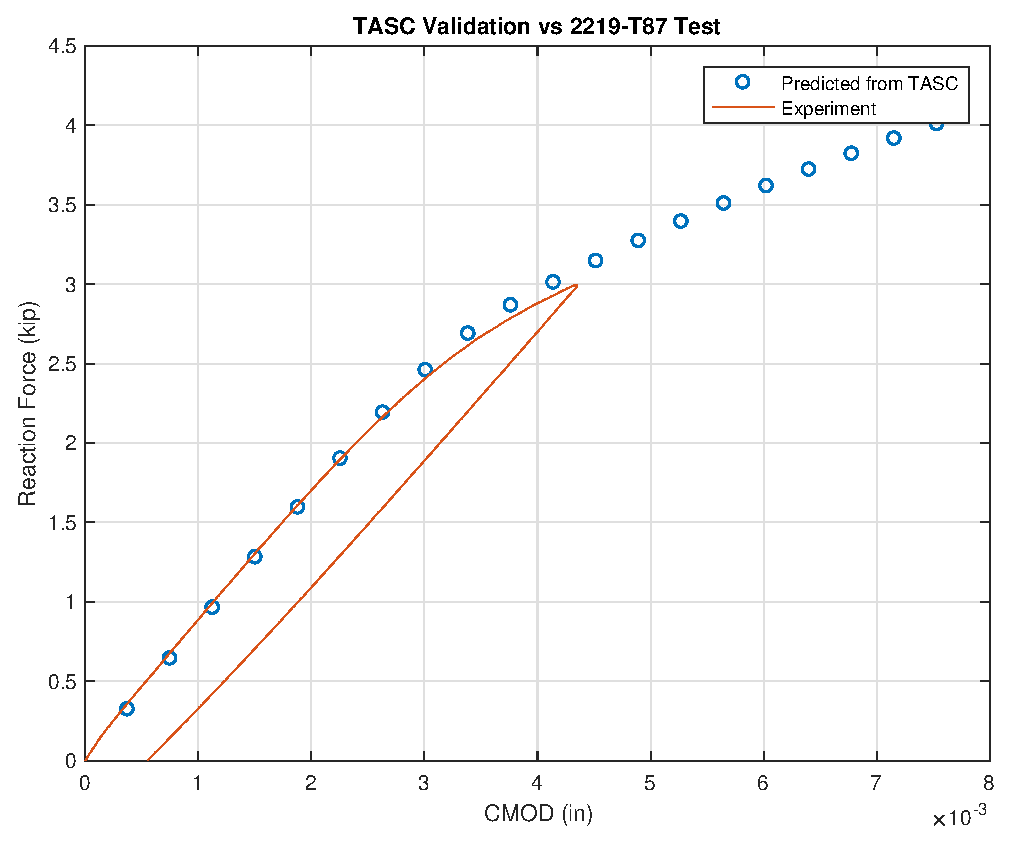
\includegraphics[width=0.7\columnwidth]{experimental-validation}
\caption{\label{fig:experimental-validation} Comparison of interpolated TASC model against bending experiment}
\end{figure}

\section{Validation of \J Values Between WARP3D and Abaqus}

Following from \Cref{sec:plan-warp-abaqus-vv}, final Abaqus files were written, and smaller models were tested interactively on a laptop virtual machine before the full set of 16 models was solved on TTU's HPC cluster.
An analytically-rigid body was constructed a planar face at \(z=0\), and serves the same purpose as the elastic boundary plane from \Cref{sec:warp-elastic-boundary}.
Frictionless contact behavior was added to the Abaqus model, and a reference point on the rigid body was fixed in all degrees of freedom.
All but two load steps created by FEACrack were deleted, leaving only the ones defining symmetry, contact, and outer roller support conditions.
A new load step was created where a displacement boundary condition derived from the WARP3D displacement results was applied to all nodes coincident with the inner roller.
The final composition of an example bending model in Abaqus can be seen in \Cref{fig:abq_bc_ac02_at02}.
\begin{sidewaysfigure}[tbp]
\centering
\includegraphics[width=\columnwidth]{{abq_bc_ac02_at02}}
\caption{\label{fig:abq_bc_ac02_at02} Example Abaqus assembly and boundary conditions (\(\frac{a}{c}=0.2\), \(\frac{a}{t}=0.2\))}
\end{sidewaysfigure}

Abaqus output databases were collected, data for \(z\) direction displacement of node 1 was used as a measure of one-half the experimental CMOD, and data for \J values at \(\phi = \) \SI{0}{\degree}, \SI{30}{\degree}, and \SI{90}{\degree} were extracted.
As seen in \Crefrange{fig:abq_wrp_ac02_at02_E0100}{fig:abq_wrp_ac10_at08_E1000}, Abaqus \J and CMOD values at \(\phi = \) \SI{30}{\degree} and \SI{90}{\degree} are nearly coincident with the values calculated in WARP3D, while the values for \(\phi = \) \SI{0}{\degree} are in close agreement except for cases of deep highly elliptical cracks \((\frac{a}{c}, \frac{a}{t})=(0.2, 0.8)\) for any material and semicircular cracks for stiff materials \((\frac{a}{c}, E) = (1.0, 1000)\).

\begin{sidewaysfigure}[tbp]
\centering
\begin{minipage}{0.49\columnwidth}
\includegraphics[width=\columnwidth]{{abq_wrp_ac02_at02_E0100_n03}}
\subcaption{\(n=3\)}
\end{minipage}%
\begin{minipage}{0.49\columnwidth}
\includegraphics[width=\columnwidth]{{abq_wrp_ac02_at02_E0100_n20}}
\subcaption{\(n=20\)}
\end{minipage}
\caption{\label{fig:abq_wrp_ac02_at02_E0100} \J comparison between Abaqus and WARP3D (\(\frac{a}{c}=0.2\), \(\frac{a}{t}=0.2\), \(E=100\))}
\end{sidewaysfigure}

\begin{sidewaysfigure}[tbp]
\centering
\begin{minipage}{0.49\columnwidth}
\includegraphics[width=\columnwidth]{{abq_wrp_ac02_at02_E1000_n03}}
\subcaption{\(n=3\)}
\end{minipage}%
\begin{minipage}{0.49\columnwidth}
\includegraphics[width=\columnwidth]{{abq_wrp_ac02_at02_E1000_n20}}
\subcaption{\(n=20\)}
\end{minipage}
\caption{\label{fig:abq_wrp_ac02_at02_E1000} \J comparison between Abaqus and WARP3D (\(\frac{a}{c}=0.2\), \(\frac{a}{t}=0.2\), \(E=1000\))}
\end{sidewaysfigure}

\begin{sidewaysfigure}[tbp]
\centering
\begin{minipage}{0.49\columnwidth}
\includegraphics[width=\columnwidth]{{abq_wrp_ac02_at08_E0100_n03}}
\subcaption{\(n=3\)}
\end{minipage}%
\begin{minipage}{0.49\columnwidth}
\includegraphics[width=\columnwidth]{{abq_wrp_ac02_at08_E0100_n20}}
\subcaption{\(n=20\)}
\end{minipage}
\caption{\label{fig:abq_wrp_ac02_at08_E0100} \J comparison between Abaqus and WARP3D (\(\frac{a}{c}=0.2\), \(\frac{a}{t}=0.8\), \(E=100\))}
\end{sidewaysfigure}

\begin{sidewaysfigure}[tbp]
\centering
\begin{minipage}{0.49\columnwidth}
\includegraphics[width=\columnwidth]{{abq_wrp_ac02_at08_E1000_n03}}
\subcaption{\(n=3\)}
\end{minipage}%
\begin{minipage}{0.49\columnwidth}
\includegraphics[width=\columnwidth]{{abq_wrp_ac02_at08_E1000_n20}}
\subcaption{\(n=20\)}
\end{minipage}
\caption{\label{fig:abq_wrp_ac02_at08_E1000} \J comparison between Abaqus and WARP3D (\(\frac{a}{c}=0.2\), \(\frac{a}{t}=0.8\), \(E=1000\))}
\end{sidewaysfigure}

\begin{sidewaysfigure}[tbp]
\centering
\begin{minipage}{0.49\columnwidth}
\includegraphics[width=\columnwidth]{{abq_wrp_ac10_at02_E0100_n03}}
\subcaption{\(n=3\)}
\end{minipage}%
\begin{minipage}{0.49\columnwidth}
\includegraphics[width=\columnwidth]{{abq_wrp_ac10_at02_E0100_n20}}
\subcaption{\(n=20\)}
\end{minipage}
\caption{\label{fig:abq_wrp_ac10_at02_E0100} \J comparison between Abaqus and WARP3D (\(\frac{a}{c}=1.0\), \(\frac{a}{t}=0.2\), \(E=100\))}
\end{sidewaysfigure}

\begin{sidewaysfigure}[tbp]
\centering
\begin{minipage}{0.49\columnwidth}
\includegraphics[width=\columnwidth]{{abq_wrp_ac10_at02_E1000_n03}}
\subcaption{\(n=3\)}
\end{minipage}%
\begin{minipage}{0.49\columnwidth}
\includegraphics[width=\columnwidth]{{abq_wrp_ac10_at02_E1000_n20}}
\subcaption{\(n=20\)}
\end{minipage}
\caption{\label{fig:abq_wrp_ac10_at02_E1000} \J comparison between Abaqus and WARP3D (\(\frac{a}{c}=1.0\), \(\frac{a}{t}=0.2\), \(E=1000\))}
\end{sidewaysfigure}

\begin{sidewaysfigure}[tbp]
\centering
\begin{minipage}{0.49\columnwidth}
\includegraphics[width=\columnwidth]{{abq_wrp_ac10_at08_E0100_n03}}
\subcaption{\(n=3\)}
\end{minipage}%
\begin{minipage}{0.49\columnwidth}
\includegraphics[width=\columnwidth]{{abq_wrp_ac10_at08_E0100_n20}}
\subcaption{\(n=20\)}
\end{minipage}
\caption{\label{fig:abq_wrp_ac10_at08_E0100} \J comparison between Abaqus and WARP3D (\(\frac{a}{c}=1.0\), \(\frac{a}{t}=0.8\), \(E=100\))}
\end{sidewaysfigure}

\begin{sidewaysfigure}[tbp]
\centering
\begin{minipage}{0.49\columnwidth}
\includegraphics[width=\columnwidth]{{abq_wrp_ac10_at08_E1000_n03}}
\subcaption{\(n=3\)}
\end{minipage}%
\begin{minipage}{0.49\columnwidth}
\includegraphics[width=\columnwidth]{{abq_wrp_ac10_at08_E1000_n20}}
\subcaption{\(n=20\)}
\end{minipage}
\caption{\label{fig:abq_wrp_ac10_at08_E1000} \J comparison between Abaqus and WARP3D (\(\frac{a}{c}=1.0\), \(\frac{a}{t}=0.8\), \(E=1000\))}
\end{sidewaysfigure}

\FloatBarrier
\section{EPRI \hone}
\label{sec:epri-results}
Following the preliminary work described in \Cref{sec:h1-verification}, a subset of the bending models were solved using Abaqus and fully-plastic checks.
The selection of elements used for the fully-plastic check in tension models was simply all elements along the crack plane, where all those elements would be subjected to a stress greater or equal to the net section stress.
However, for a bending model, some elements along the crack plane are near the neutral axis and subjected to very low stress, and other elements are in varying levels of tension or compression on either side of the neutral axis as seen in \Cref{fig:neutral-axis}.
This element set used for the fully-plastic check is in the grey region of \Cref{fig:s33-bending}, and represents the volume of material where the greatest plastic deformation occurs.

\begin{figure}[tbp]
\centering
\includegraphics[width=0.8\columnwidth]{{elements-all-fit}}
\subcaption{All elements shown for context}
\includegraphics[width=0.7\columnwidth]{{svm-limit2}}
\subcaption{Effective (von Mises) stress along crack plane, showing neutral axis for bending \label{fig:neutral-axis}}
\includegraphics[width=0.7\columnwidth]{{s33-limit2}}
\subcaption{Normal stress in \(z\) direction in crack plane, showing highest tensile stress along crack front \label{fig:s33-bending}}
\caption{\label{fig:h1_fp_check} Determination of element set used for EPRI \hone fully-plastic checks (\(\frac{a}{c}=0.2\), \(\frac{a}{t}=0.2\))}
\centering
\end{figure}
Once \J was calculated around the crack front, EPRI \hone values could be calculated with \Cref{eq:h1mcclung}.
The trend of \J values between WARP3D and Abaqus are similar at all locations along the crack front, as shown in \Cref{fig:warp_abq_j_phi_ac02_at02_E0100_n03,fig:abq_h1_ac02_at02_E0100_n03}.
As the boundary conditions sufficient to satisfy Abaqus' fully-plastic checks are higher than those required for accurate linear extrapolation of \J, the actual \J values from Abaqus are approximately double the \J values from WARP3D.
A small inflection in the \J values can be seen in both graphs near \(\phi=\SI{40}{\degree}\).
\begin{figure}[tbp]
\centering
\begin{minipage}{0.45\columnwidth}
\includegraphics[width=\columnwidth]{{bend_ac02_at02_E0100_n03_wrp_J_converge_abs}}
\subcaption{WARP3D}
\end{minipage}
\begin{minipage}{0.45\columnwidth}
\includegraphics[width=\columnwidth]{bend_ac02_at02_E0100_n03_phi_J_abq}
\subcaption{Abaqus with fully-plastic checks}
\end{minipage}
\caption{\J comparison between WARP3D model and Abaqus model with fully-plastic checks (\(\frac{a}{c}=0.2, \frac{a}{t}=0.2, E=100, n=3\)) \label{fig:warp_abq_j_phi_ac02_at02_E0100_n03}}
\end{figure}
\begin{figure}[tbp]
\centering
\includegraphics[width=0.6\columnwidth]{bend_ac02_at02_E0100_n03_phi_h1}
\caption{\hone from Abaqus model with fully-plastic checks (\(\frac{a}{c}=0.2, \frac{a}{t}=0.2, E=100, n=3\)) \label{fig:abq_h1_ac02_at02_E0100_n03}}
\end{figure}

\hone values were calculated from a subset of the WARP3D results used in the modified TASC program.
Many of the models demonstrate enough plastic deformation to make \hone independent of \(E\), and a function of geometry and hardening exponent \(n\), as seen in \Crefrange{fig:h1_warp_ac02_at02}{fig:h1_warp_ac10_at08}.
\begin{figure}[tbp]
\centering
\begin{minipage}{0.45\columnwidth}
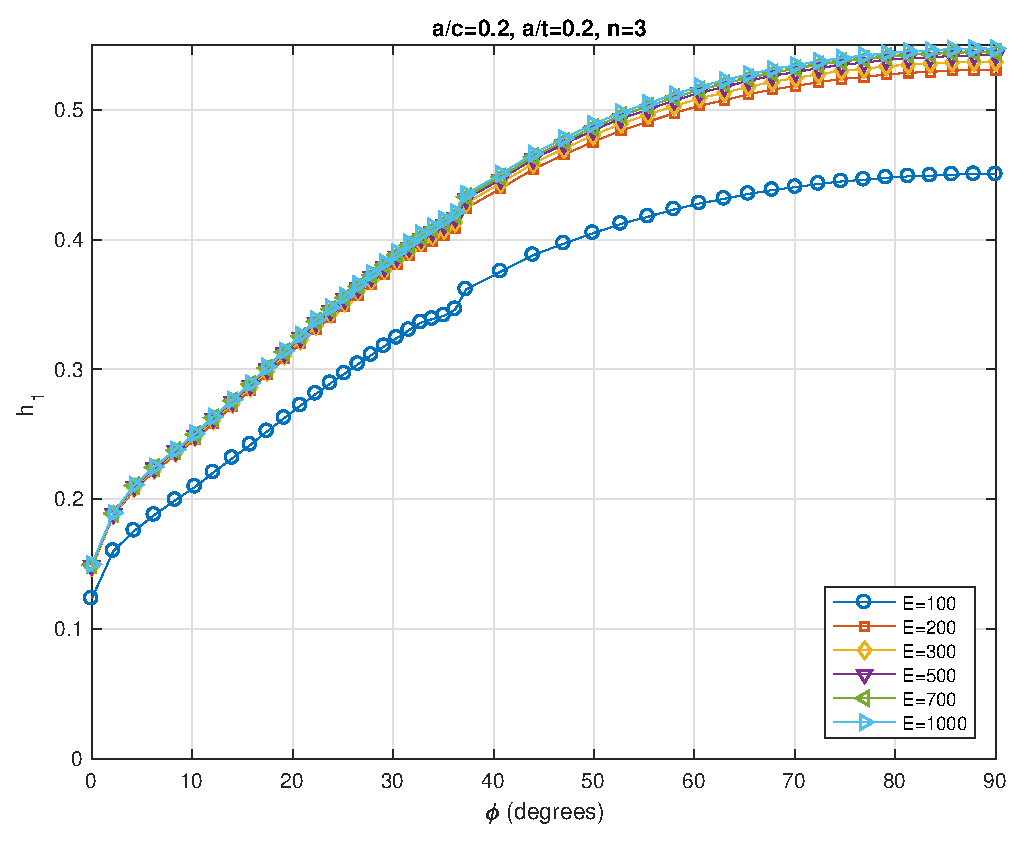
\includegraphics[width=\columnwidth]{h1_warp_ac02_at02_n03}
\subcaption{\(n=3\)}
\end{minipage}
\begin{minipage}{0.45\columnwidth}
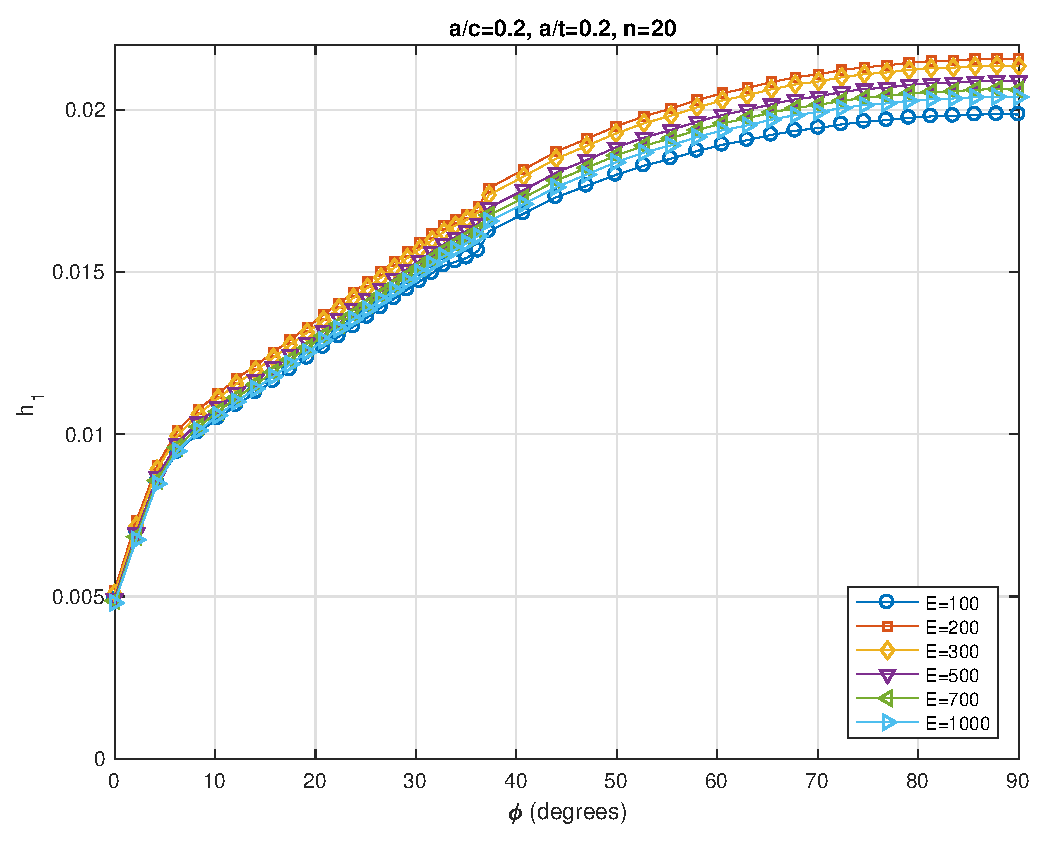
\includegraphics[width=\columnwidth]{h1_warp_ac02_at02_n20}
\subcaption{\(n=20\) \label{fig:h1_warp_ac02_at02_n20}}
\end{minipage}
\caption{\label{fig:h1_warp_ac02_at02} EPRI \hone results from WARP3D for \(\frac{a}{c}=0.2, \frac{a}{t}=0.2\)}
\end{figure}
\begin{figure}[tbp]
\centering
\begin{minipage}{0.45\columnwidth}
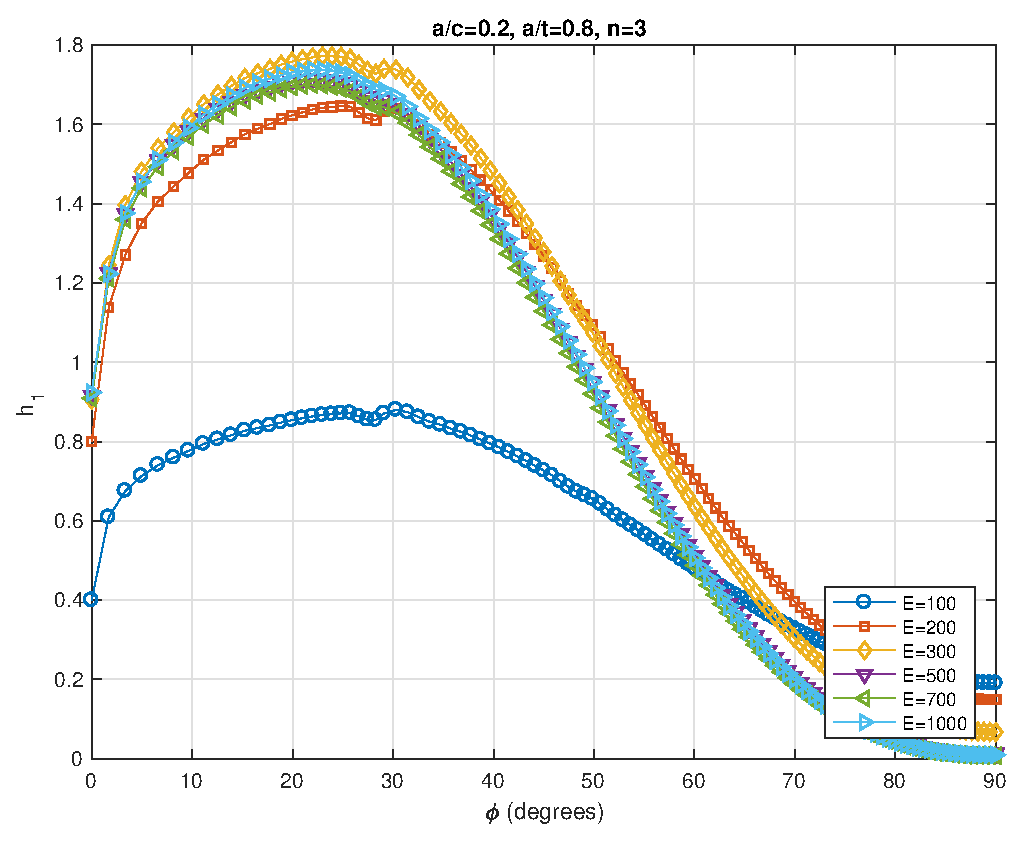
\includegraphics[width=\columnwidth]{h1_warp_ac02_at08_n03}
\subcaption{\(n=3\)}
\end{minipage}
\begin{minipage}{0.45\columnwidth}
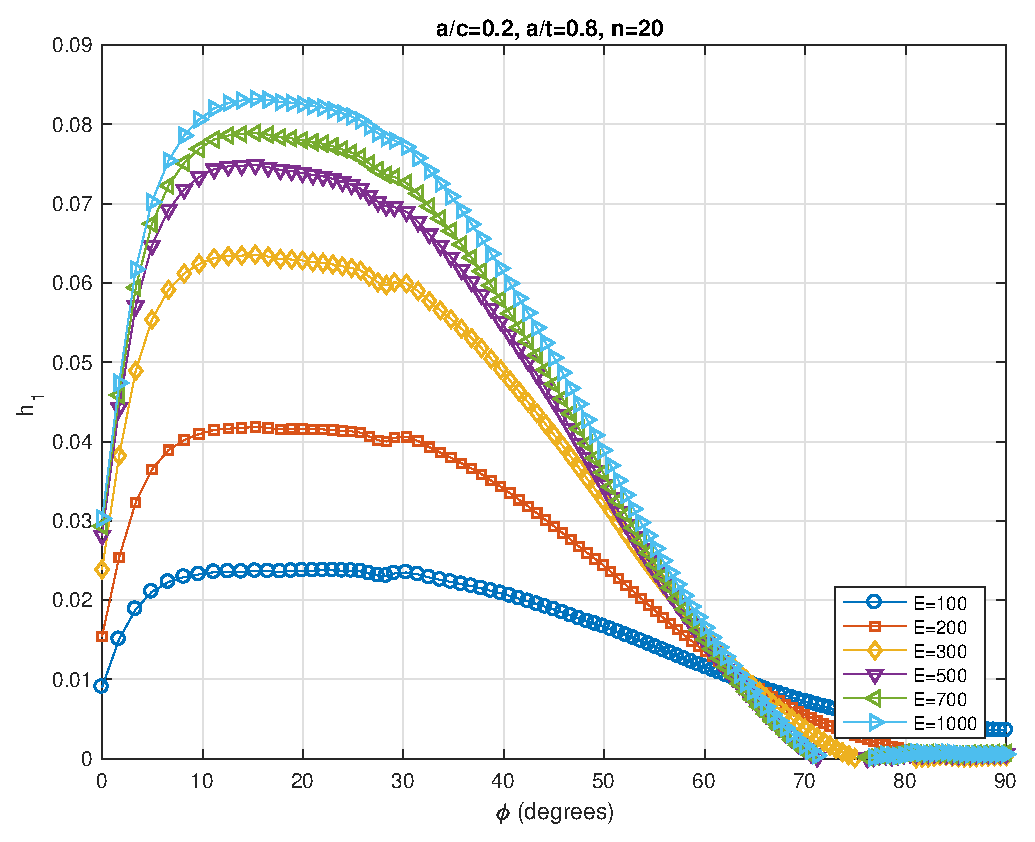
\includegraphics[width=\columnwidth]{h1_warp_ac02_at08_n20}
\subcaption{\(n=20\)}
\end{minipage}
\caption{\label{fig:h1_warp_ac02_at08} EPRI \hone results from WARP3D for \(\frac{a}{c}=0.2, \frac{a}{t}=0.8\)}
\end{figure}
\begin{figure}[tbp]
\centering
\begin{minipage}{0.45\columnwidth}
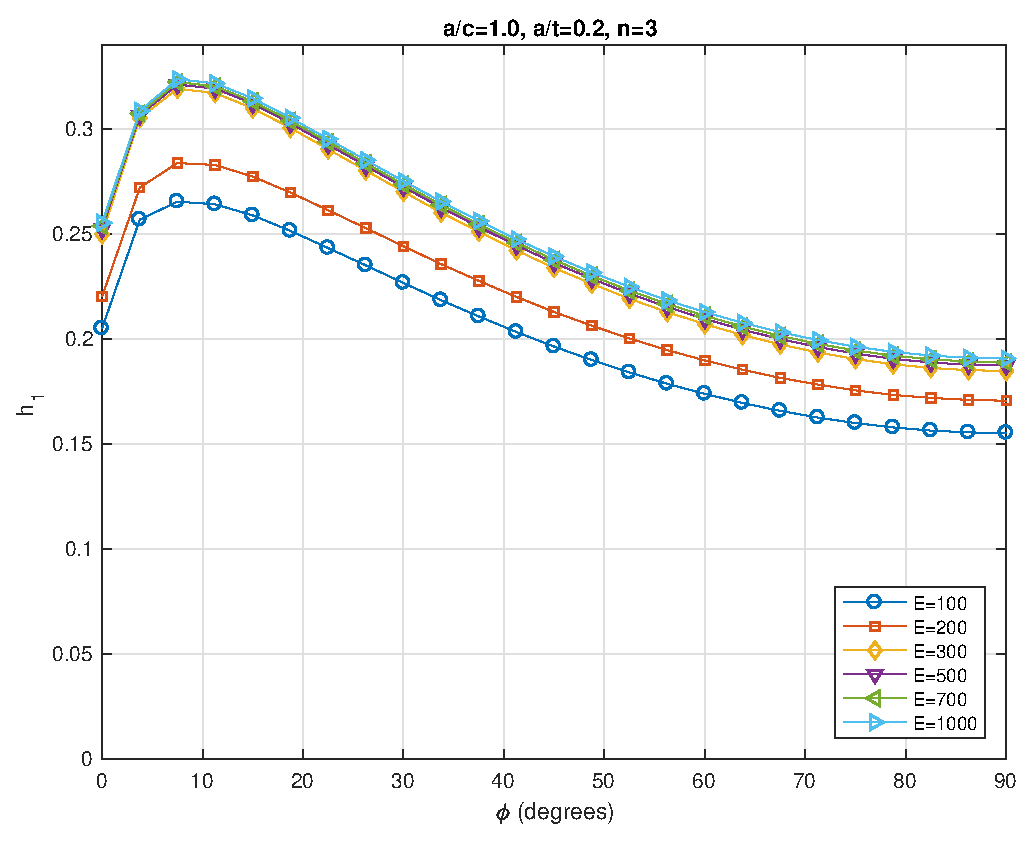
\includegraphics[width=\columnwidth]{h1_warp_ac10_at02_n03}
\subcaption{\(n=3\)}
\end{minipage}
\begin{minipage}{0.45\columnwidth}
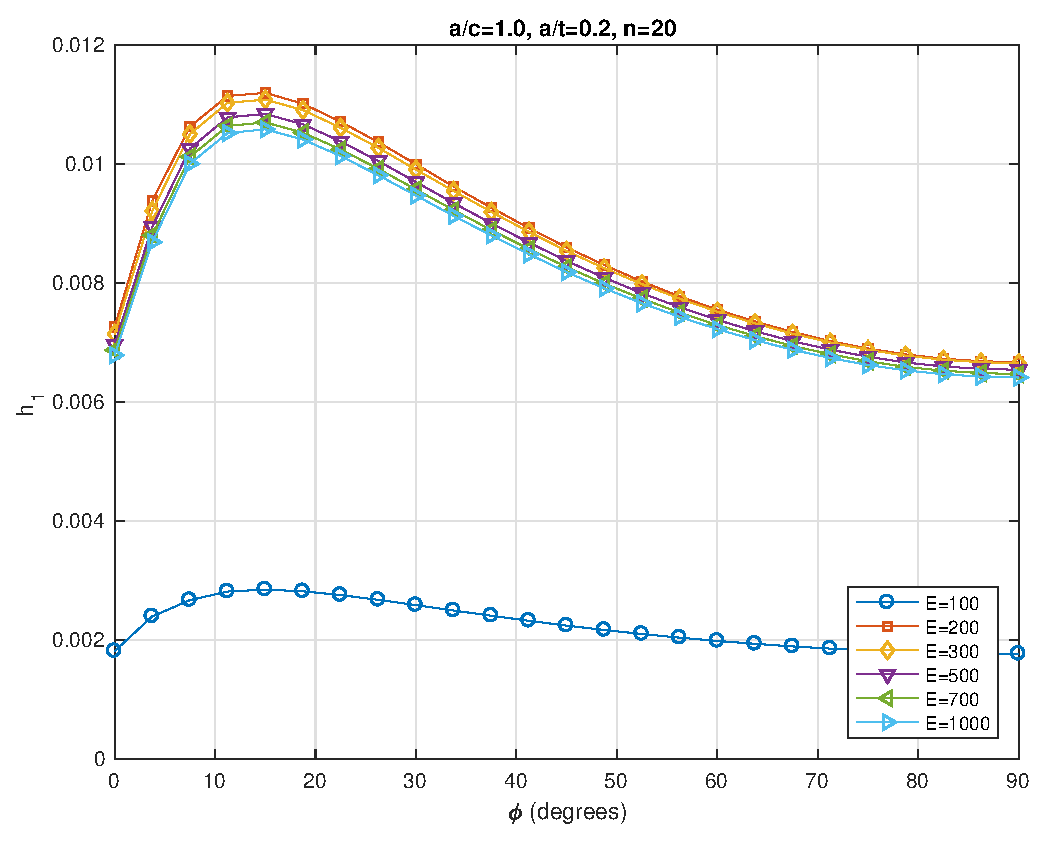
\includegraphics[width=\columnwidth]{h1_warp_ac10_at02_n20}
\subcaption{\(n=20\)}
\end{minipage}
\caption{\label{fig:h1_warp_ac10_at02} EPRI \hone results from WARP3D for \(\frac{a}{c}=1.0, \frac{a}{t}=0.2\)}
\end{figure}
\begin{figure}[tbp]
\centering
\begin{minipage}{0.45\columnwidth}
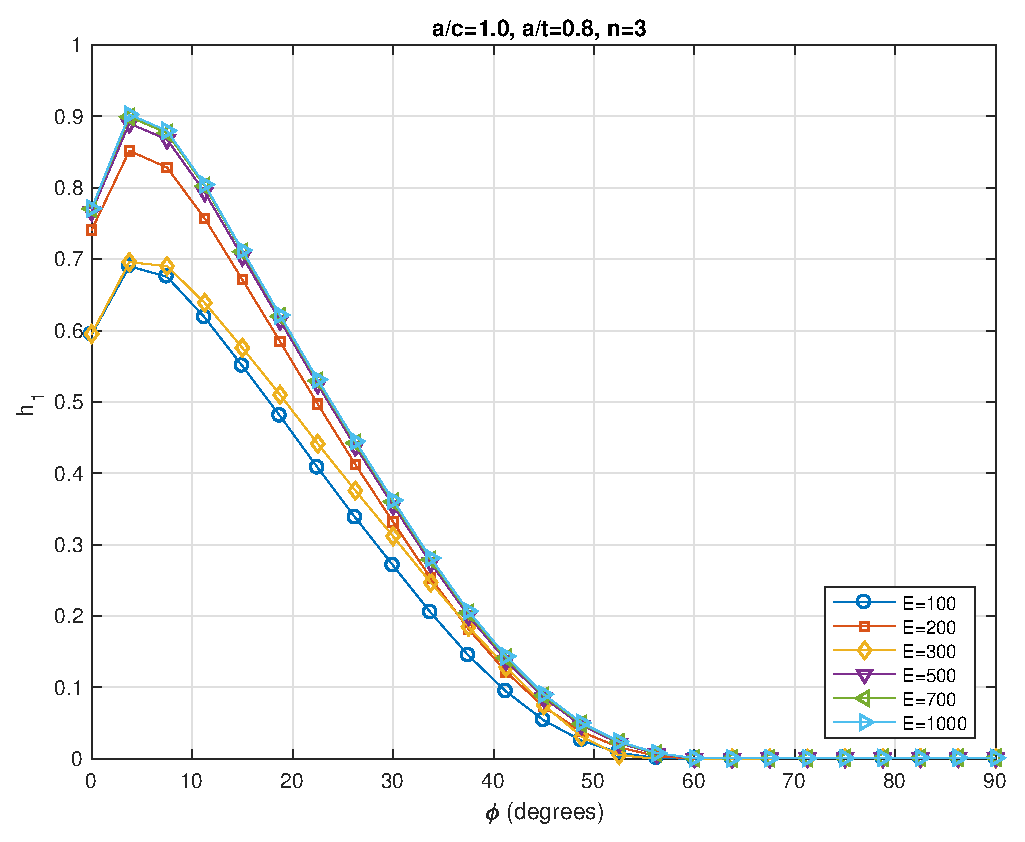
\includegraphics[width=\columnwidth]{h1_warp_ac10_at08_n03}
\subcaption{\(n=3\)}
\end{minipage}
\begin{minipage}{0.45\columnwidth}
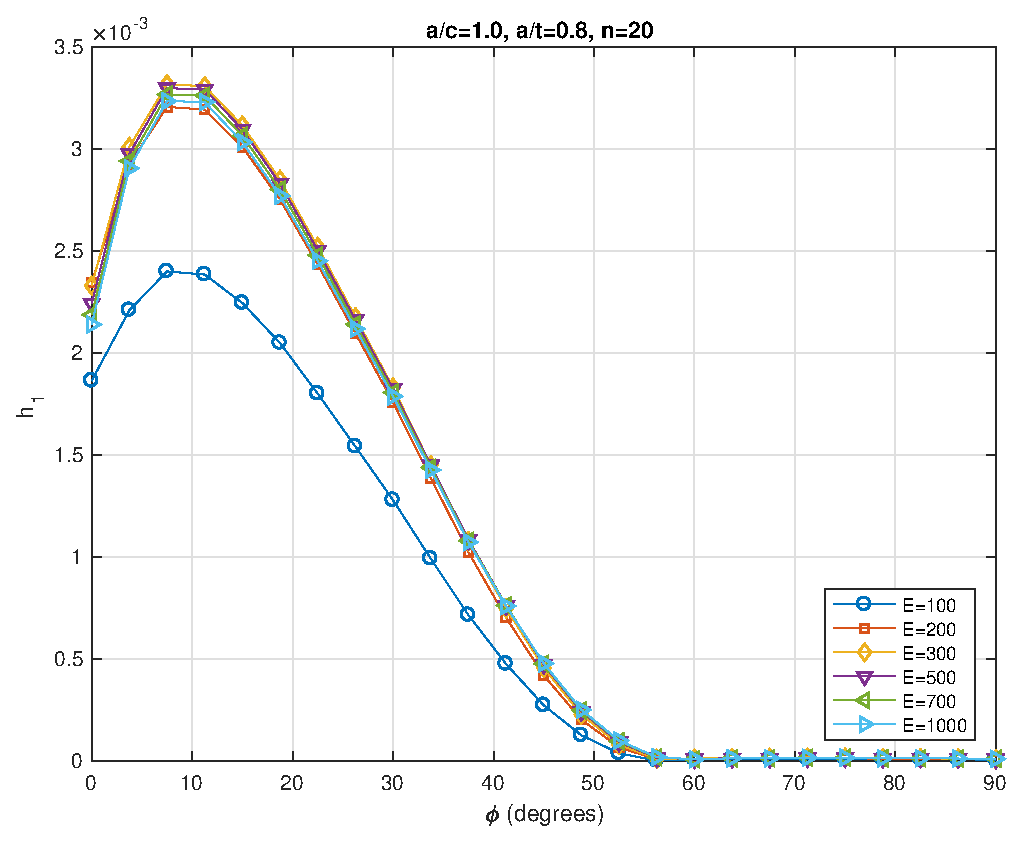
\includegraphics[width=\columnwidth]{h1_warp_ac10_at08_n20}
\subcaption{\(n=20\)}
\end{minipage}
\caption{\label{fig:h1_warp_ac10_at08} EPRI \hone results from WARP3D for \(\frac{a}{c}=1.0, \frac{a}{t}=0.8\)}
\end{figure}

\FloatBarrier
\section{Load Separation}
\label{sec:results-loadsep}

After applying the load separation technique to a set of 20 bending model results, there was no single key curve for bending, as was demonstrated in \citet{sharobeamlandes1994} for surface cracks in tension.
This led to a larger study of load separation in tension, and the discovery that the original data sets may have been too sparse to indicate the absence of a single key curve for surface cracks in tension.
At best, current results indicate that surface crack geometries are self-similar at a particular depth, but dissimilar across crack depths.

\subsection{Load Separation in Bending}

Following the methods of \citet{sharobeamlandes1994} for surface cracks in tension, the load separation technique was applied using the models' remote bending stress and CMOD.
Remote bending stress was used instead of applied force in order to compensate for the widely varying plate widths and lengths, since these could vary by a factor of 4--5, and cause similar changes in bending moment.
Similarly, the CMOD provided a much more useful localized displacement measure than the transverse displacement, since many of the shallower and narrower cracks cause little change to the plate's total compliance, and the plate width and length affects the transverse displacement under load.

Each of 20 plate geometries was run with boundary conditions large enough to cause substantial deformation as measured by the CMOD.
When the elastic component of CMOD was removed, the plastic CMOD values ranged from 0.020--0.037.
The stress-CMOD curve for the crack with dimensions \((\frac{a}{c}, \frac{a}{t})=(0.6, 0.8)\) was used as the reference curve, since it had the highest plastic CMOD value, making for easier interpolation of the \Sij separation parameter for the remaining curves.

The 20 \Sij curves ranged in value from 0.8--1.6. Since showing all 20 curves on one graph would be difficult to interpret, the family of curves is divided up by crack depth in \Crefrange{fig:Sij_at_02}{fig:Sij_at_08}.
As the earliest part of the plastic stress-CMOD curves tend to be less separable, a second set of graphs was constructed that excluded plastic CMOD values below 0.001.
Those figures are shown in \Crefrange{fig:Sij_spread_at_02}{fig:Sij_spread_at_08}.
These graphs also show the mean value of the separation parameter \Sij for each curve as a dashed line, and the deviation from that mean value.
The deviation from the mean \Sij values is given in \Cref{tab:Sij_percentage_grid}, where it can be seen that the separation parameters are consistent to within 0--3\% for \(0.6 \leq \frac{a}{t} \leq 0.8\), and within 1--6\% for \(0.2 \leq \frac{a}{t} \leq 0.4\).
As the \Sij values reported by \citeauthor{sharobeamlandes1994} were consistent to within 2\% for both surface cracks in tension and edge cracks in bending, the three-dimensional conditions and constraint effects present in surface cracks in bending have some influence on the load separation results.

\begin{figure}[tbp]
\centering
\includegraphics[width=0.8\columnwidth]{Sij_at_02}
\caption{Separation parameters for cracked plates in bending, \(\frac{a}{t}=0.2\) \label{fig:Sij_at_02}}
\end{figure}
\begin{figure}[tbp]
\centering
\includegraphics[width=0.8\columnwidth]{Sij_at_04}
\caption{Separation parameters for cracked plates in bending, \(\frac{a}{t}=0.4\) \label{fig:Sij_at_04}}
\end{figure}
\begin{figure}[tbp]
\centering
\includegraphics[width=0.8\columnwidth]{Sij_at_06}
\caption{Separation parameters for cracked plates in bending, \(\frac{a}{t}=0.6\) \label{fig:Sij_at_06}}
\end{figure}
\begin{figure}[tbp]
\centering
\includegraphics[width=0.8\columnwidth]{Sij_at_08}
\caption{Separation parameters for cracked plates in bending, \(\frac{a}{t}=0.8\) \label{fig:Sij_at_08}}
\end{figure}

\begin{figure}[tbp]
\centering
\includegraphics[width=0.8\columnwidth]{Sij_spread_at_02}
\caption{Variation of \Sij for cracked plates in bending, \(\frac{a}{t}=0.2\) \label{fig:Sij_spread_at_02}}
\end{figure}
\begin{figure}[tbp]
\centering
\includegraphics[width=0.8\columnwidth]{Sij_spread_at_04}
\caption{Variation of \Sij for cracked plates in bending, \(\frac{a}{t}=0.4\) \label{fig:Sij_spread_at_04}}
\end{figure}
\begin{figure}[tbp]
\centering
\includegraphics[width=0.8\columnwidth]{Sij_spread_at_06}
\caption{Variation of \Sij for cracked plates in bending, \(\frac{a}{t}=0.6\) \label{fig:Sij_spread_at_06}}
\end{figure}
\begin{figure}[tbp]
\centering
\includegraphics[width=0.8\columnwidth]{Sij_spread_at_08}
\caption{Variation of \Sij for cracked plates in bending, \(\frac{a}{t}=0.8\) \label{fig:Sij_spread_at_08}}
\end{figure}

\begin{table}
\caption{\label{tab:Sij_percentage_grid} Percent deviation of \Sij from mean value}
\centering
\begin{tabular}{SSSSS}
\toprule
& \multicolumn{4}{c}{\(\frac{a}{t}\)} \\
\multicolumn{1}{c}{\(\frac{a}{c}\)} & 0.2              & 0.4              & 0.6              & 0.8 \\ \cmidrule(lr){1-1} \cmidrule(lr){2-5}
0.2     & \SI{4}{\percent} & \SI{1}{\percent} & \SI{1}{\percent} & \SI{3}{\percent} \\
0.4     & \SI{5}{\percent} & \SI{1}{\percent} & \SI{0}{\percent} & \SI{1}{\percent} \\
0.6     & \SI{5}{\percent} & \SI{2}{\percent} & \SI{1}{\percent} & {N/A} \\
0.8     & \SI{6}{\percent} & \SI{3}{\percent} & \SI{1}{\percent} & \SI{0}{\percent} \\
1.0     & \SI{4}{\percent} & \SI{4}{\percent} & \SI{1}{\percent} & \SI{1}{\percent} \\ \bottomrule
\end{tabular}
\end{table}

Taking the ratio of the effective uncracked ligament to plate thickness in \cite{sharobeamlandes1994}
\begin{align}
\frac{b_e}{t} &= 1 - \frac{\pi a}{2t \left[ 2 + \frac{a/c}{a/t} \right]}
\end{align}
as a characteristic size of the crack, \Cref{fig:Sij_bet_full_E0500_n04} shows the variation of \Sij against the characteristic size.
When grouped by crack depth ratio $\frac{a}{t}$, it is clear that each group of cracks is follows a consistent trend, regardless of aspect ratio.
The curves for the shallower cracks ($0.2 \leq \frac{a}{t} \leq 0.4$) may even fall into a single larger trend, but the full set of curves does not lead to the generation of a single key curve like the one shown in \Cref{fig:sij-b-w}.
It is possible that an alternate measure of characteristic crack size could group the four curves closer together allowing a true single-specimen technique for bending, but development of this alternate measure has not yet been performed.
\begin{figure}[tbp]
\centering
\includegraphics[width=0.8\columnwidth]{Sij_bet_full_E0500_n04}
\caption{Variation of \Sij versus effective uncracked ligament length ratio (bending, \(0.2 \leq \frac{a}{t} \leq 0.8\)) \label{fig:Sij_bet_full_E0500_n04}}
\end{figure}

\subsection{Further Investigation into Load Separation in Tension}

Given the unexpected shown in \Cref{fig:Sij_bet_full_E0500_n04}, a closer investigation of load separation for surface cracks in tension was performed.
A subset of 14 tension plate models were analyzed, with crack geometry \((\frac{a}{c} \geq \frac{a}{t}, 0.2 \leq \frac{a}{t} \leq 0.8)\).
These models were quicker to analyze than the models with particularly deep elliptical cracks.
The separation parameters for the 14 plates is shown in \Cref{fig:cmodpl_Sij_tension_14}, and the variation of separation parameters across the range of effective uncracked ligament lengths is shown in \Cref{fig:bet_Sij_tension_14_annotated}.
The four models closest to the \citeauthor{sharobeamlandes1993} results have \((\frac{b_\text{e}}{t}, \Sij)\) coordinates that lie along a single line, but the tension results show the same basic trend of the bending results in \Cref{fig:Sij_bet_full_E0500_n04}: each family of cracks at a given depth have some similarity, but any trend involving cracks at different depths is at best limited to cracks of similar depths, and does not represent a trend across all crack shapes leading toward a single-specimen technique for evaluating \J.
\begin{figure}[tbp]
\centering
\includegraphics[width=0.8\columnwidth]{cmodpl_Sij_tension_14}
\caption{\label{fig:cmodpl_Sij_tension_14} Separation parameters for cracked plates in tension}
\end{figure}
\begin{figure}[tbp]
\centering
\includegraphics[width=0.8\columnwidth]{bet_Sij_tension_14_annotated}
\caption{\label{fig:bet_Sij_tension_14_annotated} Variation in \Sij versus effective uncracked ligament length (tension, \(0.2 \leq \frac{a}{t} \leq 0.8\))}
\end{figure}

\section{Summary of Results}

Conclusions and significance of the results of the current research will be detailed in \Cref{chap:conclusions}, along with recommendations for future work.
